\documentclass[border=10pt]{standalone}
\usepackage{pgfplots}
\pgfplotsset{compat=1.18}
\begin{document}
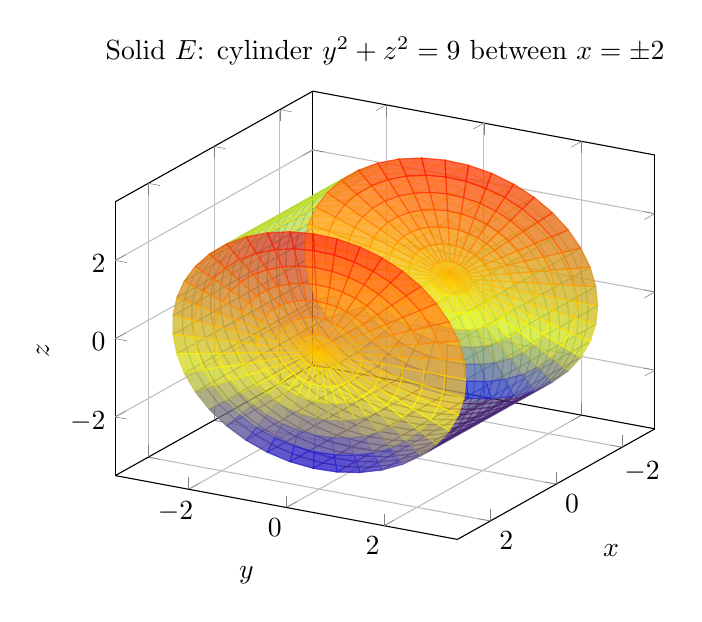
\begin{tikzpicture}
\begin{axis}[
    view={120}{25},
    xlabel={$x$}, ylabel={$y$}, zlabel={$z$},
    title={Solid $E$: cylinder $y^2+z^2=9$ between $x=\pm 2$},
    xmin=-3, xmax=3, ymin=-3.5, ymax=3.5, zmin=-3.5, zmax=3.5,
    grid=major]
% cylinder side surface
\addplot3[surf, shader=flat, opacity=0.4, colormap/viridis, domain=-2:2, y domain=0:2*pi, samples=15, samples y=40]
    ({x}, {3*cos(deg(y))}, {3*sin(deg(y))});
% end caps
\addplot3[surf, shader=flat, opacity=0.6, domain=0:3, y domain=0:2*pi, samples=8, samples y=40]
    ({-2}, {x*cos(deg(y))}, {x*sin(deg(y))});
\addplot3[surf, shader=flat, opacity=0.6, domain=0:3, y domain=0:2*pi, samples=8, samples y=40]
    ({2}, {x*cos(deg(y))}, {x*sin(deg(y))});
\end{axis}
\end{tikzpicture}
\end{document}
